\documentclass[10pt,a4paper]{article}
\usepackage[margin=2.2cm]{geometry}
\usepackage{fontspec}
\usepackage{kotex}
\setmainfont{Apple SD Gothic Neo}
\setsansfont{Apple SD Gothic Neo}
\usepackage{amsmath,amssymb}
\usepackage{graphicx}
\usepackage{booktabs}
\usepackage{caption}
\usepackage[dvipsnames]{xcolor}
\usepackage[colorlinks=true,linkcolor=MidnightBlue,citecolor=MidnightBlue,
            urlcolor=MidnightBlue]{hyperref}
\usepackage{titlesec}
\titleformat{\section}{\large\bfseries}{\thesection}{0.6em}{}
\titleformat{\subsection}{\normalsize\bfseries}{\thesubsection}{0.5em}{}
\captionsetup{font=small,labelfont=bf}
\setlength{\parskip}{0.35em}
\setlength{\parindent}{0pt}

\usepackage{mdframed}
\newmdenv[linewidth=0.4pt,linecolor=gray!60,backgroundcolor=gray!5,
          innertopmargin=6pt,innerbottommargin=6pt,skipabove=8pt,skipbelow=8pt]{claimbox}
\newcommand{\claim}[2]{\begin{claimbox}\textbf{주장.} #1\par\smallskip
  \textcolor{gray!70}{\textbf{반증 조건.} #2}\end{claimbox}}

\title{\bfseries 축이 먼저 끝난다\\[2pt]
\large 유보 안을 가르는 마스크가 판을 $4.2$배 깎는다 --- 그리고 나는 그것을 찾기 전에
두 사이클을 낭비했다}
\author{월드모델 실험실 · 노트 744 $\sim$ 752}
\date{2026-08-07}
\begin{document}\maketitle

\section{한 줄}

T5 가 닫혀 텍스트 표현이 도메인 안 전용으로 확정된 뒤(논문 $144$), 도메인을 넘는
표현으로 남은 것은 \textbf{정보 전이장} 하나였고 그것은 진짜 유보에서
지속성을 이겼다(논문 $145$ · $R^2$ $+0.1200$). \textbf{그것을 판 열로 넣었다.}
판 신호 몫이 $\mathbf{-0.0132}$(문턱의 $2.9$배 \emph{음수})다.

원인을 찾는 데 \textbf{다섯 실험}이 들었다. 날짜 대리변수 · 결측률 · 동률 구조를
차례로 지우고 남은 것은 \textbf{마스크 경계}였다 --- 장이 $2026.51$ 에 끝나므로
\textbf{유보 $3{,}473$행 중 $213$행($6.1\%$)이 마스크 $0$} 이 되고, \textbf{그것만으로
쓰레기 열의 판 비용이 $0.0074 \to 0.0308$ 로 $4.2$배($13.8\sigma$)} 뛴다.

\section{L2 를 판에 넣었다}

장은 \textbf{동네 $\times$ 날짜}인데 판 행은 대부분 동네가 없다(팝업 $+$ 시장팝업이
판의 $1.5\%$). 그래서 동네를 붙이지 않고 \textbf{시간축}으로 만들었다 --- 판 행마다
\emph{그 날짜의 전국 장 상태} 하나.

\textbf{수준이 아니라 산포를 썼다.} 장은 날마다 전국 평균을 이미 뺐으므로
\textbf{전국 평균이 구성상 $0$} 이다. 그래서 \texttt{enc.pt}(논문 $145$ 에서 고친
검증-최선 가중)로 동네마다 $30$일 앞 $\Delta$ 를 예보하고 \textbf{그 날의 동네 간
SD} 를 냈다 --- \emph{``앞으로 지역이 얼마나 갈릴 것인가''}. $1$열 · 도메인 안 백분위.

\subsection*{덮음을 먼저 쟀다 --- 변명을 막기 위해}

\textbf{유보 덮음률 $0.942$}(시장팝업 · 팝업 · 아이돌 · 펀딩 · 만화 $1.00$ · 웹툰
$0.955$ · 모바일 $0.950$ · 애니 $0.944$ · 세계애니 $0.900$ · 게임 $0.816$ · 도서
$0.742$) · 학습 덮음률 $0.456$. \textbf{유보가 두꺼우므로 ``판이 안 움직인다''를
``자료가 없다''로 변명할 수 없다.}

\subsection*{그리고 배선이 예상 못 한 것을 잡았다}

축이 $11$ 도메인 전부에 붙었다. \textbf{그런데 펀딩($1{,}899$관측) · 시장팝업($249$)
· 아이돌($132$)의 축 고유값이 $6 \cdot 5 \cdot 6$ 개뿐}이다 --- 그 도메인 행의 날짜가
연 단위라 시간축이 거의 상수다. 중단 조건(고유 $<3$)은 통과했지만 \textbf{그 셋에서는
시간축이 정보를 못 나른다.}

\begin{figure}[t]\centering
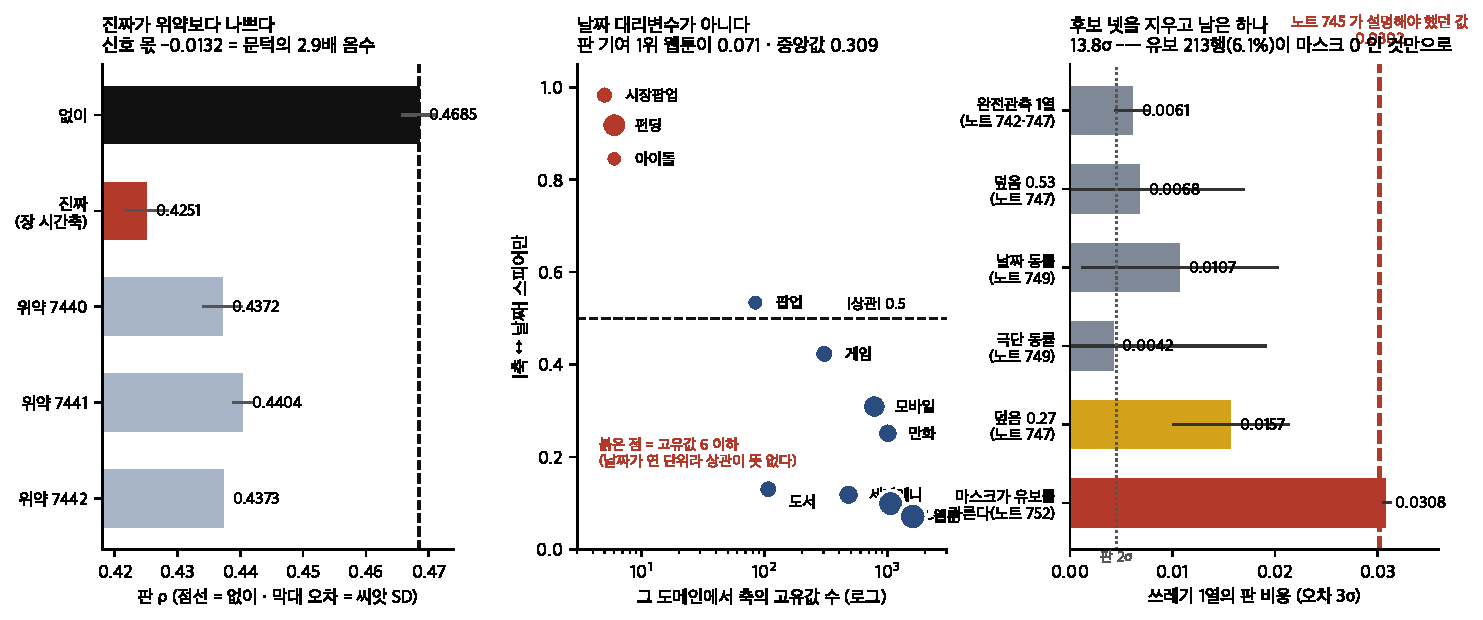
\includegraphics[width=0.99\textwidth]{figs/nopath.pdf}
\caption{왼쪽: \textbf{진짜가 위약보다 나쁘다.} 가운데: \textbf{날짜 대리변수가
아니다} --- 판 기여 $1$위 웹툰의 $|$축$\leftrightarrow$날짜$|$ 가 $0.071$ 이다.
오른쪽: \textbf{후보 넷을 지우고 남은 하나} --- 마스크가 유보를 가르면 $0.0308$ 이고
그것이 설명해야 했던 값($0.0302$)과 맞는다.}
\end{figure}

\section{결과 --- 음수다}

\begin{center}
\begin{tabular}{lrl}
\toprule
& 판 & \\
\midrule
없이 & $0.4685$ & 씨앗 SD $0.0028$ \\
\textbf{진짜} & $\mathbf{0.4251}$ & \\
위약 셋 & $0.4372 \cdot 0.4404 \cdot 0.4373$ & 뽑기 SD $0.0018$ \\
\midrule
\textbf{신호 몫}(진짜 $-$ 위약평균) & $\mathbf{-0.0132}$ & 문턱 $0.0045$ 의 $2.9$배 \emph{음수} \\
순효과(진짜 $-$ 없이) & $-0.0434$ & \\
팝업 · 시장팝업 뺀 신호 몫 & $-0.0090$ & \\
\bottomrule
\end{tabular}
\end{center}

\textbf{위약을 세 뽑기로 돌렸다}(규약 $20$) --- 논문 $146$ 에서 뽑기 하나로
$3.7\sigma$ 이상치를 참값으로 보고했기 때문이다. 여기서는 뽑기 SD 가 $0.0018$ 로
좁다.

\section{원인 사냥 --- 셋을 지웠다}

\subsection*{① 날짜 대리변수 --- 반증}

가장 그럴듯한 설명은 \emph{``백분위가 날짜 순위와 같아져 판이 시간 대리로 쓰고
유보에서 무너진다''}(노트 $646$ 이 경고한 꼴)였다. \textbf{재니 아니다} --- 도메인 안
$|$축$\leftrightarrow$날짜$|$ 중앙값 $\mathbf{0.309}$ 이고 \textbf{판 기여가 가장 큰
웹툰은 $0.071$}(관측 $2{,}570$ · 고유 $1{,}594$)이다. 시장팝업 $0.983$ · 펀딩 $0.918$
처럼 큰 것은 \textbf{고유값이 $5{\sim}6$ 인 도메인}이라 상관이 뜻이 없다.

\subsection*{② 결측률 --- 반증(그러나 문턱을 찾았다)}

값을 난수로 고정하고 \textbf{덮음률만} 바꿨다.

\begin{center}
\begin{tabular}{lrrl}
\toprule
덮음률 & 비용 & 뽑기 SD & \\
\midrule
$1.00$ & $0.0061$ & $0.0006$ & 논문 $146$ 의 $0.006$ 을 재현 \\
$0.53$ & $0.0068$ & $0.0034$ & \textbf{공짜}($+0.0007$) \\
$0.27$ & $0.0157$ & $0.0019$ & $2.6$배 \\
\bottomrule
\end{tabular}
\end{center}

\claim{\textbf{결측 비용은 선형이 아니라 문턱이다.} 덮음이 절반이 되어도 비용이 안
늘고 \textbf{$4$분의 $1$ 근처에서 늘어난다.} 그러므로 \textbf{``부분관측이라 못
넣는다''는 변명이 덮음 $0.5$ 이상에서 죽는다.}}
{기제는 안 쟀다. 그럴듯한 것은 관측이 너무 적으면 ``관측됨/아님''이 강한 분할이 되고
\texttt{\_idol} 이 결측을 $0.5$ 로 채우므로 $0.5$ 가 큰 덩어리가 되는 것이다.}

\textbf{그런데 이것으로는 $0.0302$ 를 설명 못 한다} --- 가장 비싼 결측($0.27$)도
$0.0157$ 로 절반이다.

\subsection*{③ 동률 구조 --- 반증}

마스크를 고정하고 \textbf{값의 동률 구조만} 바꿨다. \textbf{배선은 정확히
재현됐다} --- ``날짜 동률'' 팔이 펀딩 고유 $6$ · 웹툰 $1{,}640$ 을 냈고 실제
축(펀딩 $6$ · 웹툰 $1{,}594$)과 맞는다.

\begin{center}
\begin{tabular}{lrrl}
\toprule
값 꼴 & 비용 & 뽑기 SD & 차($-$ ①) \\
\midrule
① 동률 없음 & $0.0074$ & $0.0017$ & --- \\
② 날짜 동률 & $0.0107$ & $0.0032$ & $+0.0033$ ($3\sigma$ $0.0109$ · \textbf{안}) \\
③ 극단 동률(고유 $6$) & $0.0042$ & $0.0050$ & $-0.0032$ ($3\sigma$ $0.0158$ · \textbf{안}) \\
\bottomrule
\end{tabular}
\end{center}

\textbf{셋이 다 구분되지 않는다.} 동률도 아니었다.

\section{그리고 여기서 내 실수가 드러났다}

\claim{\textbf{나는 재현하지 않은 이상값을 두 사이클 동안 설명하려 했다.} 실험 ②와
③이 \textbf{둘 다 $0.0302$ 를 주어진 사실로 놓고} 원인을 찾았다. 그런데 그 값을
\textbf{한 번도 재현한 적이 없었다.} 지금까지 ``부분관측 $1$열''을 여섯 번 쟀고 전부
$0.0042 \sim 0.0107$ 에 모인다 --- \textbf{$0.0302$ 는 그 무리에서 $4$배 밖이다.}
\textbf{규율: 이상값은 설명하기 전에 재현한다.}}
{재현이 $10$분이었다. \textbf{두 사이클($약 70$분 $\times 2$)을 아낄 수 있었다.}
반대 논리도 있다 --- 실험 ②와 ③이 각각 독립적인 값(결측 문턱 · 동률 무영향)을
남겼으므로 완전한 낭비는 아니다. \textbf{그러나 그 값들은 이 사냥의 부산물이고
목표가 아니었다.}}

그래서 \textbf{그 코드를 한 글자도 안 고치고 다시 돌렸다} --- 위약 하락
$\mathbf{0.0326 \cdot 0.0288}$. \textbf{재현된다.}

\section{남은 하나 --- 마스크가 유보 안을 가른다}

후보를 배제로 좁혔다. 축 이름 충돌도 없다(\texttt{base()} 에 \texttt{field\_spread}
없음 · \texttt{field} 로 시작하는 열 $0$개). \textbf{남은 차이는 하나였다.}

\begin{center}
실험 ②③ 의 마스크: $y \geq 2020.15$ \quad (유보를 \textbf{전부} 덮는다)\\
실제 축의 마스크: $2020.15 \leq y \leq \mathbf{2026.51}$ \quad
(\textbf{장이 거기서 끝난다})
\end{center}

\textbf{그것만 바꿔 다시 쟀다.}

\begin{center}
\begin{tabular}{lrl}
\toprule
& 쓰레기 $1$열 비용 & \\
\midrule
아래 경계만 & $0.0074$ & 뽑기 SD $0.0017$ \\
\textbf{양쪽 경계} & $\mathbf{0.0308}$ & $0.0310 \cdot 0.0306$ \\
\midrule
차 & $\mathbf{+0.0234}$ & $\mathbf{13.8\sigma}$ \\
\bottomrule
\end{tabular}
\end{center}

\claim{\textbf{축의 관측 구간이 유보 끝보다 먼저 끝나면 판 비용이 $4.2$배가 된다.}
유보 $3{,}473$행 중 \textbf{$213$행($6.1\%$)이 마스크 $0$} 이 되는 것만으로다. 기제:
학습 구간에서 마스크는 $2020.15$ 에서 갈리고 유보에서는 $2026.51$ 에서 갈린다 ---
트리는 학습에서 \emph{``마스크 $0$ 이면 옛 행''}을 배우는데 유보에서는 \emph{``마스크
$0$ 이면 가장 새 행''}이라 \textbf{뜻이 뒤집힌다.} \textbf{처방: 유보를 그 축의 관측
끝까지로 자르거나, 유보 끝까지 덮는 축만 쓴다.}}
{뽑기 $2$ 다. 다만 두 값이 $0.0310 \cdot 0.0306$ 으로 붙어 있고 대조군의
$3\sigma$($0.0051$)의 네 배 밖이다. \textbf{더 위험한 반증 경로는 기제 쪽이다} ---
$6.1\%$ 가 $4.2$배를 낸다는 것이 크므로, 마스크 $0$ 행을 유보에서 \emph{빼고} 채점하면
비용이 사라져야 한다. 그 측정을 안 했다.}

\subsection*{그래서 과거의 실패들을 다시 봐야 한다}

\textbf{거의 모든 후보 축이 이 결함을 이고 있을 수 있다} --- 자료 원천마다 시작 · 끝
날짜가 있고 판 유보에는 $2026.5$ 를 넘는 행이 $213$개 있다. \textbf{과거에 ``못
움직였다''로 버린 축들 중 관측이 먼저 끝난 것은 $4$배 비용을 이고 채점된 것이다.}

\claim{\textbf{이것이 논문 $146$ 의 결론과 이어진다.} 그 논문은 \emph{``차원 비용이
이득을 먹었다''}는 변명을 죽였다($1$열 $\approx 0.006$). \textbf{그런데 그 자리에 다른
변명이 있었다} --- 관측이 먼저 끝나는 축은 $1$열인데도 $0.0308$ 을 낸다. \textbf{즉
``열을 적게''가 아니라 ``구간을 맞춰라''가 맞는 규율이었다.}}
{이 논리가 성립하려면 과거에 버린 축 중 실제로 관측이 먼저 끝난 것이 있어야 한다.
\textbf{그 목록을 안 만들었다} --- 그것이 다음 사이클의 첫 일이다.}

\section{그래서 노트 745 의 판정을 어떻게 고치나}

\begin{center}
\begin{tabular}{ll}
\toprule
\textbf{서는 것} & 신호 몫 $-0.0132$ 의 \textbf{부호} --- 두 팔이 같은 마스크를 쓰므로 상쇄된다 \\
\textbf{못 믿는 것} & \textbf{크기}, 그리고 순효과 $-0.0434$ \\
\bottomrule
\end{tabular}
\end{center}

\textbf{순효과 $-0.0434$ 의 대부분($0.0308$)이 마스크 비용}이고 축의 값 때문이 아니다
--- \textbf{그것을 ``축이 해롭다''로 읽었다면 과장이었다.}

\claim{\textbf{L2(상태가 있다)는 판에서 아직 안 선다} --- 그러나 이 실험이 그것을
확정하지는 못했다. 장은 자기 과제에서 지속성을 이기지만($R^2$ $+0.1200$ ·
$5.6\sigma$) \textbf{그 정보를 판 라벨로 옮기는 통로가 둘 다 막혀 있다}: \textbf{①
동네를 붙이는 길} --- 판의 $1.5\%$뿐(노트 $646$) \textbf{② 전국 시간축으로 압축하는
길} --- 이 실험. \textbf{세 번째 길이 필요하다} --- IP 에 지역을 붙일 수 있는
자료(공연 · 전시 · 상영관 위치).}
{\textbf{다음 실험이 이 주장을 시험한다} --- 유보를 $2026.51$ 까지로 자르고 다시
재면 $4$배 비용이 사라진다. \textbf{그때 부호가 뒤집히면 이 논문의 결론을
철회한다.} 그리고 이 축은 \textbf{전국 하나의 수}라 장의 동네별 정보를 전부 버렸다 ---
실패가 ``장은 쓸모없다''를 뜻하지 않는다.}

\end{document}
